\documentclass[lang=cn,11pt,a4paper,cite=authornum]{paper}

\title{Linux开发环境及应用 上机作业一:正则表达式应用 \\ 实验报告}
\author{毛子恒 \\ 2019211397}
\institute{北京邮电大学\ 计算机学院}

\date{\zhtoday}

\setmonofont{Consolas}

% 本文档命令
\nocite{*}

\begin{document}

\maketitle

\section{实验内容}

从因特网上搜索Web页,用\mintinline{text}{wget}获取网页,处理网页HTML文本数据,从中提取出当前时间点北京各监测站的PM2.5浓度,输出CSV格式数据。

\section{实验步骤}

\paragraph{获取数据}

使用命令\mintinline{text}{wget http://www.86pm25.com/city/beijing.html -o /dev/null}取得数据,结果保存在\mintinline{text}{beijing.html}中。

\paragraph{去除HTML标签}

使用命令\mintinline{text}{sed -e 's/<[^<>]*>/ /g'},去除其中的HTML标签,其中的正则表达式匹配以尖括号包含的、其中不含尖括号的字符串。

\paragraph{获取时间和处理数据}

去除标签之后,得到的数据表格如\figref{fig:p1}。

\begin{figure}[!htb]
    \centering
    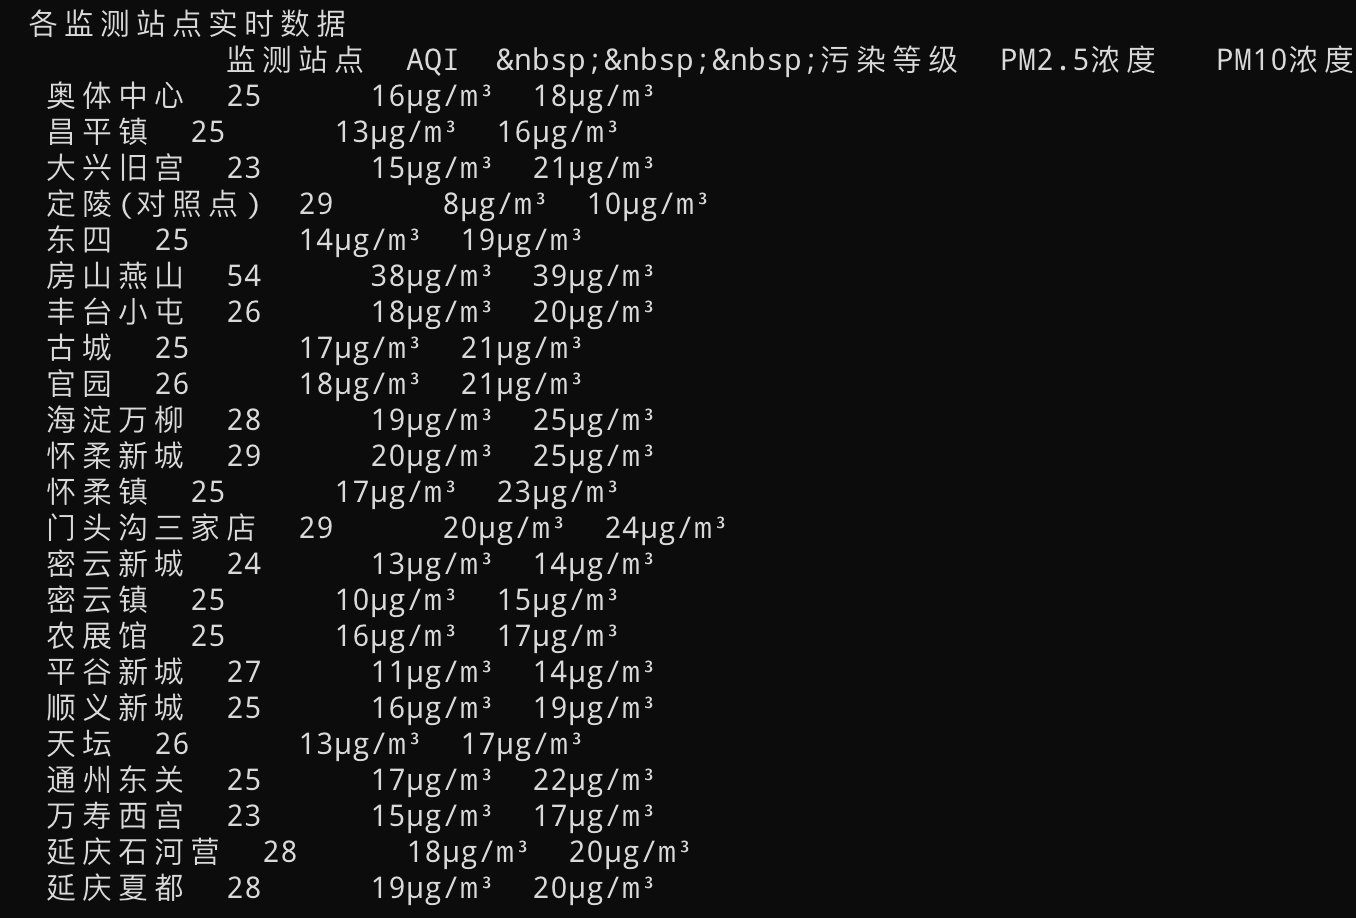
\includegraphics[width=\textwidth]{./images/l1-p1.jpg}
    \caption{\label{fig:p1}}
\end{figure}

另外可以找到时间信息如“更新:2022年03月19日 11时”,日期在第一个区域,小时在第二个区域。

因此,采用“更新”关键词获取到时间,之后对于每一个包含\mintinline{text}{μg/m³}的行,气象站地点在第一个区域,PM2.5的值在第三个区域,调整格式并打印,最后编写的awk文件如下:

\begin{code}
    \begin{minted}{text}
/更新/{ date = $1; time = $2;}
/μg\/m³/{printf("%s %s:00:00,%s,%s\n", date, time, $1, $3);}
\end{minted}
\end{code}

使用命令\mintinline{text}{awk -f work.awk},得到的数据表格如\figref{fig:p2}。

\begin{figure}[!htb]
    \centering
    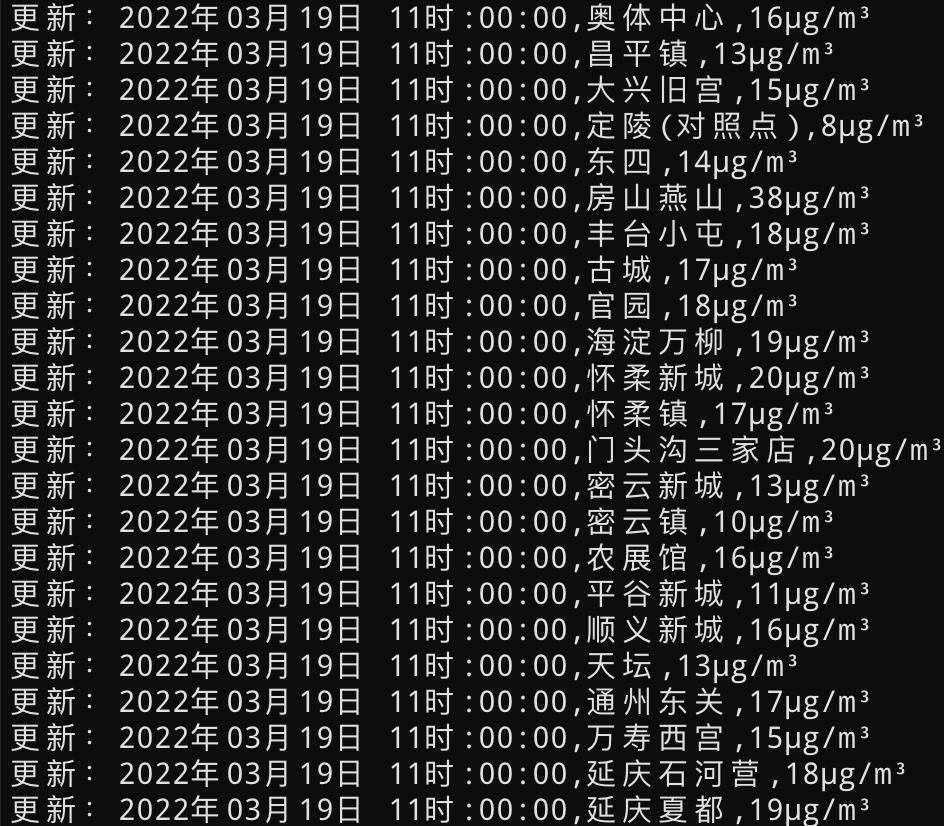
\includegraphics[width=0.7\textwidth]{./images/l1-p2.jpg}
    \caption{\label{fig:p2}}
\end{figure}

\paragraph{调整格式}

去掉“更新”二字,调整时间格式为\mintinline{text}{yyyy-mm-dd hh:00:00},去掉\mintinline{text}{μg/m³},使用命令\mintinline{text}{sed -e 's/更新://g' -e 's/\([0-9]*\)年\([0-9]*\)月\([0-9]*\)日/\1-\2-\3/g' -e 's/时//g' -e 's/μg\/m³//g'}。

\paragraph{输出到文件}

使用命令\mintinline{text}{tee result.csv >/dev/null}输出到\mintinline{text}{result.csv},最终结果如\figref{fig:p3}。

\begin{figure}[!htb]
    \centering
    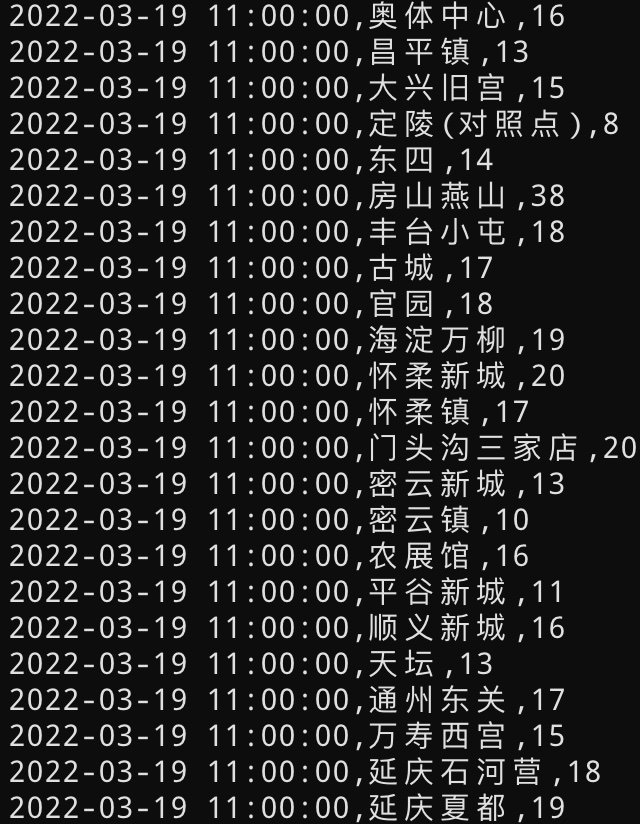
\includegraphics[width=0.5\textwidth]{./images/l1-p3.jpg}
    \caption{\label{fig:p3}}
\end{figure}

所有命令连起来如\figref{fig:p4}。

\begin{figure}[!htb]
    \centering
    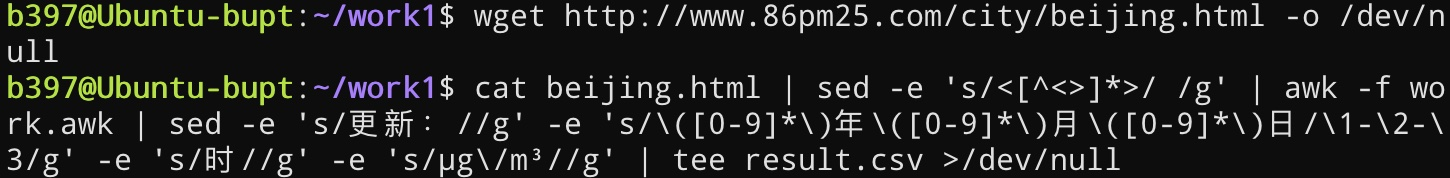
\includegraphics[width=\textwidth]{./images/l1-p4.jpg}
    \caption{\label{fig:p4}}
\end{figure}

\section{实验总结}

本次实验中我熟悉了\mintinline{text}{sed,awk,tee}等命令的功能和正则表达式的基本语法,并且成功运用它们处理了简单的文本文件。

\end{document}